% Options for packages loaded elsewhere
\PassOptionsToPackage{unicode}{hyperref}
\PassOptionsToPackage{hyphens}{url}
\PassOptionsToPackage{dvipsnames,svgnames,x11names}{xcolor}
%
\documentclass[
  letterpaper,
  DIV=11,
  numbers=noendperiod]{scrartcl}

\usepackage{amsmath,amssymb}
\usepackage{lmodern}
\usepackage{iftex}
\ifPDFTeX
  \usepackage[T1]{fontenc}
  \usepackage[utf8]{inputenc}
  \usepackage{textcomp} % provide euro and other symbols
\else % if luatex or xetex
  \usepackage{unicode-math}
  \defaultfontfeatures{Scale=MatchLowercase}
  \defaultfontfeatures[\rmfamily]{Ligatures=TeX,Scale=1}
\fi
% Use upquote if available, for straight quotes in verbatim environments
\IfFileExists{upquote.sty}{\usepackage{upquote}}{}
\IfFileExists{microtype.sty}{% use microtype if available
  \usepackage[]{microtype}
  \UseMicrotypeSet[protrusion]{basicmath} % disable protrusion for tt fonts
}{}
\makeatletter
\@ifundefined{KOMAClassName}{% if non-KOMA class
  \IfFileExists{parskip.sty}{%
    \usepackage{parskip}
  }{% else
    \setlength{\parindent}{0pt}
    \setlength{\parskip}{6pt plus 2pt minus 1pt}}
}{% if KOMA class
  \KOMAoptions{parskip=half}}
\makeatother
\usepackage{xcolor}
\setlength{\emergencystretch}{3em} % prevent overfull lines
\setcounter{secnumdepth}{-\maxdimen} % remove section numbering
% Make \paragraph and \subparagraph free-standing
\ifx\paragraph\undefined\else
  \let\oldparagraph\paragraph
  \renewcommand{\paragraph}[1]{\oldparagraph{#1}\mbox{}}
\fi
\ifx\subparagraph\undefined\else
  \let\oldsubparagraph\subparagraph
  \renewcommand{\subparagraph}[1]{\oldsubparagraph{#1}\mbox{}}
\fi


\providecommand{\tightlist}{%
  \setlength{\itemsep}{0pt}\setlength{\parskip}{0pt}}\usepackage{longtable,booktabs,array}
\usepackage{calc} % for calculating minipage widths
% Correct order of tables after \paragraph or \subparagraph
\usepackage{etoolbox}
\makeatletter
\patchcmd\longtable{\par}{\if@noskipsec\mbox{}\fi\par}{}{}
\makeatother
% Allow footnotes in longtable head/foot
\IfFileExists{footnotehyper.sty}{\usepackage{footnotehyper}}{\usepackage{footnote}}
\makesavenoteenv{longtable}
\usepackage{graphicx}
\makeatletter
\def\maxwidth{\ifdim\Gin@nat@width>\linewidth\linewidth\else\Gin@nat@width\fi}
\def\maxheight{\ifdim\Gin@nat@height>\textheight\textheight\else\Gin@nat@height\fi}
\makeatother
% Scale images if necessary, so that they will not overflow the page
% margins by default, and it is still possible to overwrite the defaults
% using explicit options in \includegraphics[width, height, ...]{}
\setkeys{Gin}{width=\maxwidth,height=\maxheight,keepaspectratio}
% Set default figure placement to htbp
\makeatletter
\def\fps@figure{htbp}
\makeatother

\KOMAoption{captions}{tableheading}
\makeatletter
\makeatother
\makeatletter
\makeatother
\makeatletter
\@ifpackageloaded{caption}{}{\usepackage{caption}}
\AtBeginDocument{%
\ifdefined\contentsname
  \renewcommand*\contentsname{Table of contents}
\else
  \newcommand\contentsname{Table of contents}
\fi
\ifdefined\listfigurename
  \renewcommand*\listfigurename{List of Figures}
\else
  \newcommand\listfigurename{List of Figures}
\fi
\ifdefined\listtablename
  \renewcommand*\listtablename{List of Tables}
\else
  \newcommand\listtablename{List of Tables}
\fi
\ifdefined\figurename
  \renewcommand*\figurename{Figure}
\else
  \newcommand\figurename{Figure}
\fi
\ifdefined\tablename
  \renewcommand*\tablename{Table}
\else
  \newcommand\tablename{Table}
\fi
}
\@ifpackageloaded{float}{}{\usepackage{float}}
\floatstyle{ruled}
\@ifundefined{c@chapter}{\newfloat{codelisting}{h}{lop}}{\newfloat{codelisting}{h}{lop}[chapter]}
\floatname{codelisting}{Listing}
\newcommand*\listoflistings{\listof{codelisting}{List of Listings}}
\makeatother
\makeatletter
\@ifpackageloaded{caption}{}{\usepackage{caption}}
\@ifpackageloaded{subcaption}{}{\usepackage{subcaption}}
\makeatother
\makeatletter
\@ifpackageloaded{tcolorbox}{}{\usepackage[many]{tcolorbox}}
\makeatother
\makeatletter
\@ifundefined{shadecolor}{\definecolor{shadecolor}{rgb}{.97, .97, .97}}
\makeatother
\makeatletter
\makeatother
\ifLuaTeX
  \usepackage{selnolig}  % disable illegal ligatures
\fi
\IfFileExists{bookmark.sty}{\usepackage{bookmark}}{\usepackage{hyperref}}
\IfFileExists{xurl.sty}{\usepackage{xurl}}{} % add URL line breaks if available
\urlstyle{same} % disable monospaced font for URLs
\hypersetup{
  pdftitle={Informe de regresión lineal simple y múltiple: Resumen, Laboratorio Capítulos 2 y 3 ( An Introduction to Statistical Learning)},
  pdfauthor={Mariuxi Maribel Tenesaca Yuqui},
  colorlinks=true,
  linkcolor={blue},
  filecolor={Maroon},
  citecolor={Blue},
  urlcolor={Blue},
  pdfcreator={LaTeX via pandoc}}

\title{Informe de regresión lineal simple y múltiple: Resumen,
Laboratorio Capítulos 2 y 3 ( An Introduction to Statistical Learning)}
\author{Mariuxi Maribel Tenesaca Yuqui}
\date{}

\begin{document}
\maketitle
\ifdefined\Shaded\renewenvironment{Shaded}{\begin{tcolorbox}[boxrule=0pt, frame hidden, breakable, borderline west={3pt}{0pt}{shadecolor}, sharp corners, interior hidden, enhanced]}{\end{tcolorbox}}\fi

\hypertarget{capuxedtulo-2-aprendizaje-estaduxedstico}{%
\subsection{Capítulo 2: Aprendizaje
Estadístico}\label{capuxedtulo-2-aprendizaje-estaduxedstico}}

\emph{El aprendizaje estadístico se refiere a un conjunto de enfoques
para estimar f.}

\begin{itemize}
\item
  Un ejemplo de un estudio de aprendizaje estadístico que investiga la
  correlación entre la publicidad y las ventas de productos en
  diferentes mercados.
\item
  Los datos de publicidad y ventas se tabulan y se busca un modelo
  preciso para pronosticar las ventas en función de los presupuestos de
  publicidad en televisión, radio y periódicos.
\item
  ~El presupuesto de publicidad es la variable de entrada (o
  independiente) etiquetada como X1, X2 y X3, mientras que las ventas
  son la variable de salida (o dependiente) etiquetada como Y.
\item
  Los términos ``predictor'', ``variable independiente'', ``función'' o
  simplemente ``variable''. '' se usan indistintamente para referirse a
  la variable de entrada, mientras que la variable de salida también se
  puede llamar ``respuesta'' o ``variable dependiente''.
\end{itemize}

\hypertarget{por-quuxe9-estimar-f}{%
\subsubsection{\texorpdfstring{\textbf{¿Por qué estimar
f?}}{¿Por qué estimar f?}}\label{por-quuxe9-estimar-f}}

Hay dos razones principales por las que podemos querer estimar f:

\begin{enumerate}
\def\labelenumi{\arabic{enumi}.}
\item
  Predicción
\item
  Inferencia
\end{enumerate}

\textbf{Predicción}

En muchas situaciones, se dispone fácilmente de un conjunto de entradas
X, pero la salida Y no puede obtenerse fácilmente.

En este caso, Dado que el término de error tiene un valor medio a cero,
podemos predecir Y utilizando

Yˆ = ˆf(X),

\begin{itemize}
\item
  Donde ˆf representa nuestra estimación para f
\item
  Yˆ representa la predicción resultante para Y .
\item
  En este entorno, ˆf suele tratarse como una caja negra, en el sentido
  de que en el sentido de que a uno no le suele preocupar la forma
  exacta de ˆf, siempre y cuando produzca predicciones precisas para Y.
\end{itemize}

\hypertarget{interferencia}{%
\subsubsection{\texorpdfstring{\textbf{Interferencia}}{Interferencia}}\label{interferencia}}

En este contexto, se puede predecir Y utilizando una estimación para f,
y Y representa la predicción resultante para Y.

Si el objetivo es entender la asociación entre Y y X1,...,Xp, se debe
estimar f, pero no necesariamente para hacer predicciones para Y. En
este caso, no se puede tratar ˆf como una caja negra, ya que se necesita
conocer su forma exacta.

Algunas preguntas que pueden surgir son:

\begin{itemize}
\tightlist
\item
  ¿Qué predictores se asocian a la respuesta?
\end{itemize}

~A menudo que sólo una pequeña fracción de los predictores disponibles
están con Y

\begin{itemize}
\tightlist
\item
  ¿Cuál es la relación entre la respuesta y cada predictor?
\end{itemize}

\begin{enumerate}
\def\labelenumi{\arabic{enumi}.}
\item
  Algunos predictores pueden tener una relación positiva con Y.
\item
  La relación entre la respuesta y un predictor.
\item
  También puede depender de los valores de los demás predictores.
\end{enumerate}

\begin{itemize}
\tightlist
\item
  ¿Puede resumirse adecuadamente la relación entre Y y cada predictor
  utilizando una ecuación lineal, o es la relación más complicada?
\end{itemize}

Históricamente, la mayoría de los métodos para estimar f han adoptado
una forma lineal.

\emph{En algunos casos, se pueden modelar la predicción y la
inferencia.}

Dependiendo del objetivo final de nuestro análisis, pueden ser
apropiados diferentes métodos para estimar f.

\begin{itemize}
\tightlist
\item
  Por ejemplo, los modelos lineales permiten inferencias relativamente
  simples e interpretables, pero es posible que no proporcionen
  predicciones tan precisas como algunos métodos no lineales.
\end{itemize}

\hypertarget{cuxf3mo-estimamos-f}{%
\subsubsection{\texorpdfstring{\textbf{¿Cómo estimamos
f?}}{¿Cómo estimamos f?}}\label{cuxf3mo-estimamos-f}}

Siempre supondremos que hemos observado un conjunto de n puntos de datos
diferentes puntos de datos. Por ejemplo, en la Figura 1 observamos n =
30 puntos de datos.

\begin{figure}

{\centering 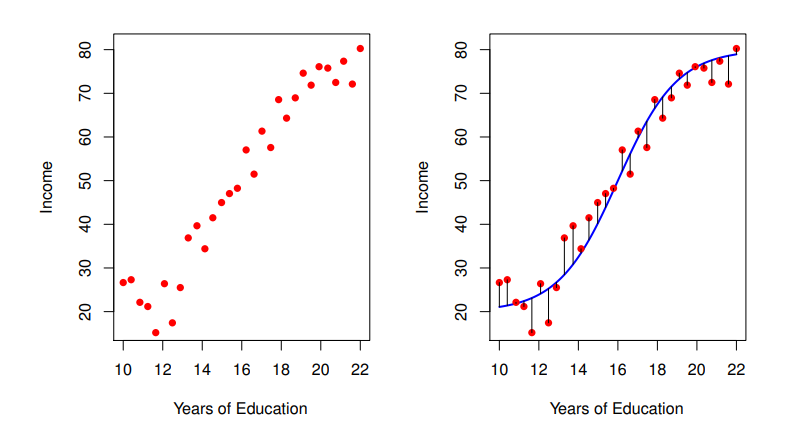
\includegraphics[width=2.97917in,height=\textheight]{images/figura1.png}

}

\end{figure}

Estas observaciones se denominan datos de entrenamiento, ya se usarán
para:

\begin{itemize}
\tightlist
\item
  Entrenar o enseñar.
\end{itemize}

Para entrenar, o enseñar, a nuestro método a estimar f.

\begin{itemize}
\tightlist
\item
  yi representa la variable de respuesta de la i-ésima observación.
\end{itemize}

Los datos de entrenamiento son:

\begin{itemize}
\tightlist
\item
  \{(x1, y1),(x2, y2),...,(xn, yn)\} donde xi = (xi1, xi2,...,xip)T .
\end{itemize}

Nuestro objetivo es aplicar un método de aprendizaje estadístico a los
datos de entrenamiento

para estimar la función desconocida f.

\begin{itemize}
\tightlist
\item
  Es decir encontrar una función ˆf tal que Y ≈ ˆf(X) para cualquier
  observación (X, Y ). En términos generales
\end{itemize}

\hypertarget{muxe9todos-paramuxe9tricos}{%
\subsubsection{\texorpdfstring{\textbf{Métodos
paramétricos}}{Métodos paramétricos}}\label{muxe9todos-paramuxe9tricos}}

Los métodos paramétricos implican un enfoque basado en modelos de dos
pasos.

\emph{La forma funcional}

Por ejemplo, una suposición muy sencilla es que f es lineal en X:

f(X) = β0 + β1X1 + β2X2 + -\/-\/- + βpXp

Después de seleccionar un modelo, se necesita un procedimiento que use
los datos de entrenamiento para ajustar o entrenar el modelo. En el caso
del modelo lineal, necesitamos estimar los parámetros β0, β1,..., βp
para encontrar los valores que ajusten los datos.

Es decir, queremos encontrar valores de estos parámetros tales que

Y ≈ β0 + β1X1 + β2X2 + -\/-\/- + βpXp.

El enfoque más común para ajustar el modelo lineal es el método de
mínimos cuadrados ordinarios.

\hypertarget{muxe9todos-no-paramuxe9tricos}{%
\subsubsection{\texorpdfstring{\textbf{Métodos no
paramétricos}}{Métodos no paramétricos}}\label{muxe9todos-no-paramuxe9tricos}}

Los métodos no paramétricos no hacen suposiciones explícitas sobre la
forma funcional de f.

En su lugar, buscan una estimación de f que se acerque lo más posible a
los puntos de datos sin que sea demasiado aproximada u ondulada.

Los puntos de datos sin ser demasiado aproximados o imprecisos.

Los enfoques no paramétricos no se hace ninguna suposición sobre la
forma de f.~Sin embargo, los enfoques no paramétricos tienen una gran
desventaja.

Desventaja: dado que no reducen el problema de estimar f a un numero de
parámetros, se necesita un gran número de observaciones (muchas más de
las que se suelen necesitar para un método paramétrico).

En la Figura 2 se muestra un ejemplo de ajuste no paramétrico de los
datos de ingresos.

\begin{figure}

{\centering 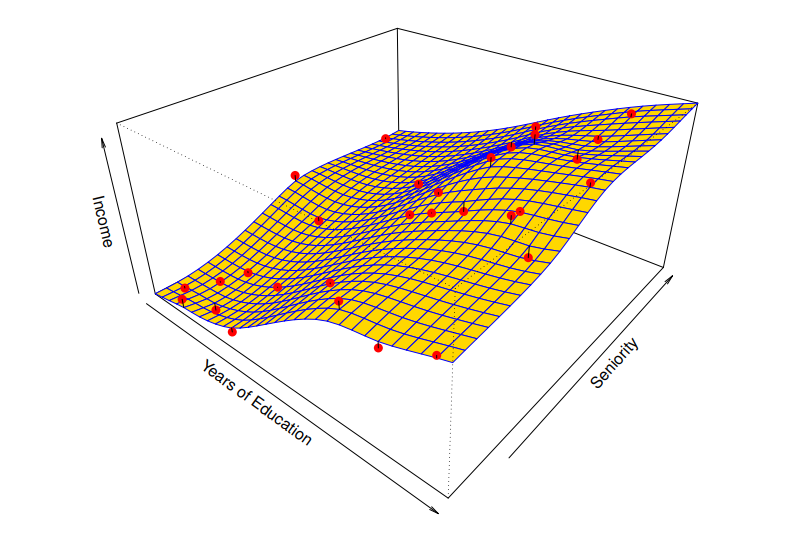
\includegraphics[width=3.40625in,height=\textheight]{images/figura2.png}

}

\caption{En amarillo se muestra un ajuste suave de placa delgada a los
datos de Ingresos.}

\end{figure}

\hypertarget{el-equilibrio-entre-la-precisiuxf3n-de-la-predicciuxf3n-y-la-interpretabilidad-del-modelo}{%
\subsubsection{\texorpdfstring{\textbf{El equilibrio entre la precisión
de la predicción y la interpretabilidad del
modelo}}{El equilibrio entre la precisión de la predicción y la interpretabilidad del modelo}}\label{el-equilibrio-entre-la-precisiuxf3n-de-la-predicciuxf3n-y-la-interpretabilidad-del-modelo}}

\begin{itemize}
\item
  La regresión lineal es un enfoque relativamente inflexible, porque
  sólo puede generar funciones lineales.
\item
  Otros métodos, como los splines de placa delgada: Son
  considerablemente más flexibles porque pueden generar una gama de
  formas posibles para estimar f.
\end{itemize}

\textbf{¿Por qué utilizar un método más restrictivo en lugar de un
enfoque más flexible?}

\emph{Hay varias razones por las que podríamos preferir un modelo más
restrictivo.}

Si nos interesa principalmente la inferencia, los modelos restrictivos
son mucho más interpretables.

\begin{itemize}
\tightlist
\item
  Por ejemplo, cuando el objetivo es la inferencia, el modelo lineal
  lineal puede ser una buena elección, ya que será bastante fácil
  entender la relación entre Y y X1, X2,...,Xp.
\end{itemize}

En general, a medida que aumenta la flexibilidad de un método, disminuye
su interpretabilidad.

\begin{figure}

{\centering 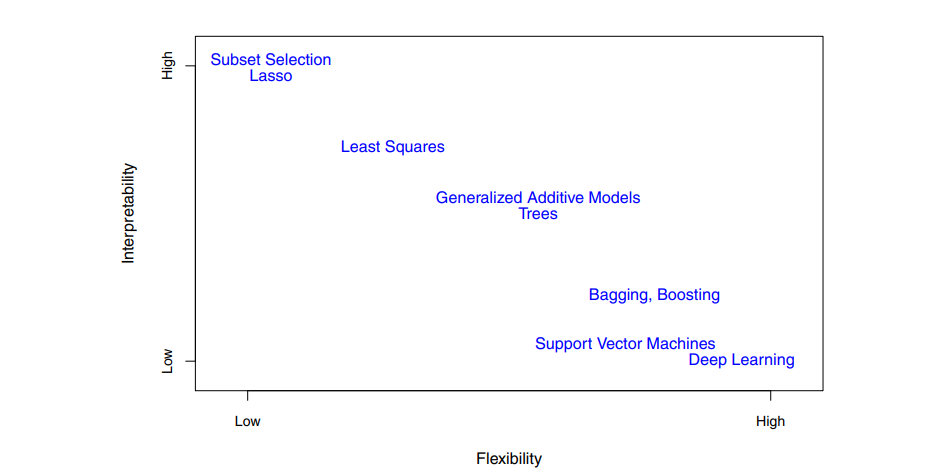
\includegraphics[width=4.29167in,height=\textheight]{images/figura3.png}

}

\caption{Una representación del compromiso entre flexibilidad e
interpretabilidad, utilizando diferentes métodos de aprendizaje
estadístico.}

\end{figure}

\hypertarget{aprendizaje-supervisado-frente-a-aprendizaje-no-supervisado}{%
\subsubsection{\texorpdfstring{\textbf{Aprendizaje supervisado frente a
aprendizaje no
supervisado}}{Aprendizaje supervisado frente a aprendizaje no supervisado}}\label{aprendizaje-supervisado-frente-a-aprendizaje-no-supervisado}}

La mayoría de los problemas de aprendizaje estadístico pertenecen a una
de estas dos categorías: \textbf{supervisados o no supervisados}.

\begin{itemize}
\tightlist
\item
  Para cada observación de predictor(es) xi, i = 1,...,n hay una medida
  de respuesta asociada yi de respuesta yi.
\end{itemize}

Objetivo: Ajustar un modelo que relacione la respuesta con los
predictores, con el fin de predecir con exactitud la respuesta para
futuras de la (predicción) o comprender mejor la relación entre la
respuesta y los predictores.

\emph{Métodos clásicos de aprendizaje estadístico que operan en el
ámbito de la supervisión:}

\begin{enumerate}
\def\labelenumi{\arabic{enumi}.}
\item
  Regresión lineal
\item
  La regresión logística
\item
  GAM
\item
  Boosting
\item
  Máquinas de regresión de vec- soporte
\end{enumerate}

\begin{itemize}
\tightlist
\item
  El aprendizaje no supervisado describe la situación algo más difícil
  en la que para cada observación i = 1,...,n.
\end{itemize}

Ejemplo: Un vector de medidas xi, pero ninguna respuesta asociada yi. No
es posible ajustar un modelo de regresión lineal, ya que no existe una
variable de respuesta

\begin{itemize}
\item
  En este contexto, en cierto modo trabajamos a ciegas
\item
  La situación se denomina no supervisada porque carecemos de una
  variable de respuesta que pueda supervisar nuestro análisis.
\end{itemize}

\hypertarget{problemas-de-regresiuxf3n-frente-a-problemas-de-clasificaciuxf3n}{%
\subsubsection{\texorpdfstring{\textbf{Problemas de regresión frente a
problemas de
clasificación}}{Problemas de regresión frente a problemas de clasificación}}\label{problemas-de-regresiuxf3n-frente-a-problemas-de-clasificaciuxf3n}}

En estadística, las variables pueden ser cuantitativas o cualitativas
(también conocidas como categóricas). Las variables cuantitativas toman
valores numéricos, mientras que las variables cualitativas toman valores
de diferentes categorías.

Los problemas con una variable de respuesta cuantitativa se denominan
problemas de regresión, mientras que los problemas con una variable de
respuesta cualitativa se denominan problemas de clasificación. Sin
embargo, la distinción no siempre es clara, ya que en ambos casos se
pueden utilizar ciertos métodos, como la regresión logística.

La elección del método de aprendizaje estadístico viene determinada por
la variable respuesta (cuantitativa o cualitativa), mientras que el tipo
de variable predictora (cualitativa o cuantitativa) se considera
secundaria.

Independientemente del tipo de predictor, la mayoría de las técnicas de
aprendizaje estadístico se pueden utilizar siempre que los predictores
cualitativos estén codificados correctamente antes del análisis.

\hypertarget{evaluaciuxf3n-de-la-precisiuxf3n-de-los-modelos}{%
\subsubsection{\texorpdfstring{\textbf{Evaluación de la precisión de los
modelos}}{Evaluación de la precisión de los modelos}}\label{evaluaciuxf3n-de-la-precisiuxf3n-de-los-modelos}}

Ningún método único es adecuado para todos los conjuntos de datos
posibles, por lo que es importante elegir el método apropiado para cada
conjunto de datos en particular.

\hypertarget{medir-la-calidad-del-ajuste}{%
\subsubsection{\texorpdfstring{\textbf{Medir la calidad del
ajuste}}{Medir la calidad del ajuste}}\label{medir-la-calidad-del-ajuste}}

Para evaluar el rendimiento de un método de aprendizaje estadístico en
un conjunto de datos determinado, necesitamos algún modo de medir hasta
qué punto sus predicciones:

Se necesita cuantificar hasta qué punto medida en que el valor de
respuesta predicho para una observación dada se aproxima el verdadero
valor de respuesta para esa observación.

En el ámbito de la regresión, la medida más utilizada es el error
cuadrático medio (ECM), dado por:

\begin{figure}

{\centering 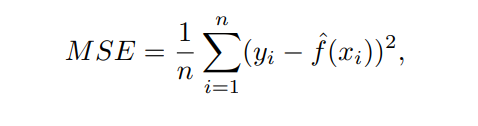
\includegraphics[width=2.70833in,height=\textheight]{images/figura4.png}

}

\end{figure}

\begin{itemize}
\item
  ˆf(xi) es la predicción que da ˆf para la i-ésima observación. El MSE
  será pequeño si las respuestas predichas están muy cerca de las
  respuestas verdaderas.
\item
  Será grande si las respuestas pronosticadas y verdaderas para algunas
  observaciones difieren significativamente.
\end{itemize}

El error cuadrático medio (MSE) se calcula utilizando los datos de
entrenamiento utilizados para ajustar el modelo, por lo que debería
llamarse MSE de entrenamiento con mayor precisión. Pero, en general, no
nos importa qué tan bien funciona el método en los datos de
entrenamiento.

En cambio, estamos interesados \hspace{0pt}\hspace{0pt}en la precisión
de las predicciones que obtenemos al aplicar nuestro método a datos de
prueba nunca antes vistos. Esto es importante porque nos interesa cómo
manejará el método los datos futuros, no cómo manejará los datos pasados
\hspace{0pt}\hspace{0pt}que se usaron para entrenar el modelo.

En la práctica, suele ser fácil calcular el MSE de entrenamiento:

\begin{itemize}
\item
  Estimar el MSE de prueba es mucho más difícil porque los datos de
  prueba generalmente no están disponibles.
\item
  El nivel de elasticidad correspondiente al modelo con el MSE de prueba
  más pequeño puede variar significativamente entre los conjuntos de
  datos.
\item
  Un enfoque importante es la validación cruzada, que es un método
  cruzado que utiliza datos de entrenamiento para estimar el MSE de una
  prueba.
\end{itemize}

\hypertarget{la-relaciuxf3n-entre-sesgo-y-varianza}{%
\subsubsection{\texorpdfstring{\textbf{La relación entre sesgo y
varianza}}{La relación entre sesgo y varianza}}\label{la-relaciuxf3n-entre-sesgo-y-varianza}}

Es posible demostrar que el MSE de prueba esperado, para un valor dado
x0, siempre puede descomponerse en la suma de los valores de x0 y x0.

Siempre puede descomponerse en la suma de tres cantidades fundamentales:
la varianza de ˆf(x0), el sesgo al cuadrado de ˆf(x0) y la varianza del
error error ϵ. Es decir:

\begin{figure}

{\centering 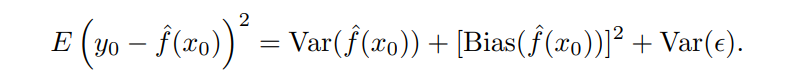
\includegraphics[width=3.82292in,height=0.39583in]{images/figura5.png}

}

\end{figure}

La notación E (Y0 - ˆf(x0) define el MSE de prueba esperado en x0, se
refiere al MSE de prueba medio que obtendríamos si probáramos
repetidamente MSE.

Se estima f utilizando un gran número de conjuntos de entrenamiento.

El término ``varianza'' se refiere a la cantidad en la que cambiaría la
estimación de f si se usara un conjunto de datos de entrenamiento
diferente para estimarla.

En general, los métodos estadísticos más flexibles marcan una mayor
diferencia.

Si el método tiene una varianza alta, pequeños cambios en los datos de
entrenamiento pueden causar grandes cambios en la estimación de \^{}f.

La mayor flexibilidad de un modelo estadístico afecta su varianza y
sesgo y cómo esto afecta las pruebas de MSE.

A medida que aumenta la elasticidad, el sesgo tiende a disminuir más
rápido que la varianza, lo que hace que disminuya el MSE de la prueba
inicial. Pero después de cierto punto, la varianza aumenta
significativamente y el MSE de la prueba comienza a aumentar.

La relación entre el sesgo, la varianza y el MSE del conjunto de prueba
que se da en la ecuación y se muestra en la figura 6 se denomina
compromiso sesgo-varianza.

\begin{figure}

{\centering 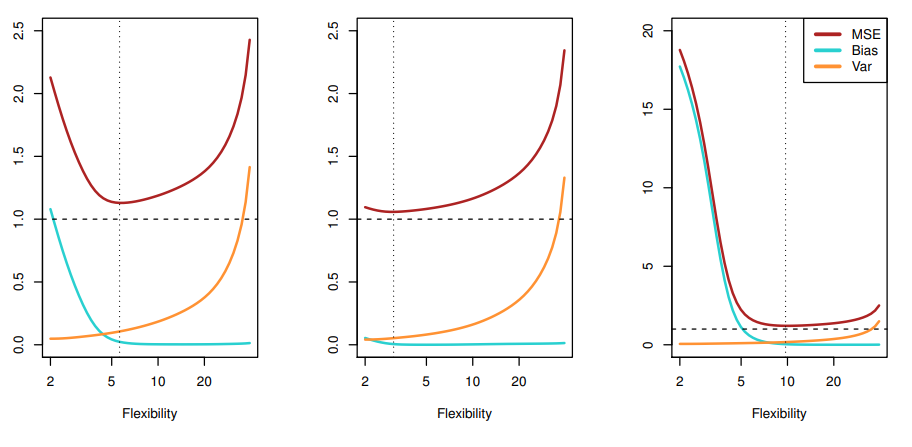
\includegraphics[width=3.5in,height=\textheight]{images/figura6-01.png}

}

\end{figure}

La relación entre sesgo y varianza es conocida como compromiso
sesgo-varianza.

Para lograr un buen rendimiento del conjunto de prueba de un método de
aprendizaje estadístico es necesario encontrar un equilibrio entre una
varianza baja y un sesgo al cuadrado bajo. Esto es difícil de lograr ya
que es fácil obtener métodos con baja varianza, pero alto sesgo o
métodos con bajo sesgo, pero alta varianza.

Encontrar un método con ambos baja varianza y sesgo al cuadrado bajo es
un desafío importante en el aprendizaje estadístico.

\textbf{El entorno de clasificación}

Muchos de los conceptos que hemos encontrado, como como el equilibrio
entre sesgo y varianza, se transfieren al entorno de clasificación con
sólo algunas modificaciones debidas al hecho de que yi ya no es
cuantitativo.

Supongamos que queremos estimar f a partir de observaciones de
entrenamiento \{(x1, y1),...,(xn, yn)\}, donde ahora y1,...,yn son
cualitativas.

El enfoque más común para cuantificar la precisión de nuestra estimación
ˆf es la tasa de error de entrenamiento, la proporción de errores que se
cometen si aplicamos la tasa de error nuestra estimación ˆf a las
observaciones de entrenamiento:

\begin{figure}

{\centering 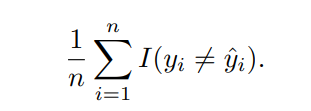
\includegraphics[width=1.85417in,height=\textheight]{images/figura7.png}

}

\end{figure}

\hypertarget{el-clasificador-de-bayes}{%
\subsubsection{\texorpdfstring{\textbf{El clasificador de
Bayes}}{El clasificador de Bayes}}\label{el-clasificador-de-bayes}}

Simplemente hay que asignar una observación de prueba con el vector
predictor x0 a la clase j para la que:

\begin{figure}

{\centering 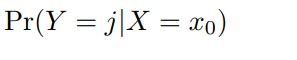
\includegraphics[width=1.73958in,height=\textheight]{images/figura8.png}

}

\end{figure}

Es una probabilidad condicional: probabilidad de que Y = j, dado el
vector predictor observado x0.

Este clasificador tan sencillo se denomina clasificador de Bayes. En un
problema de dos clases en el que sólo hay dos posibles valores de
respuesta, la clase 1 o la clase 2.

\begin{figure}

{\centering 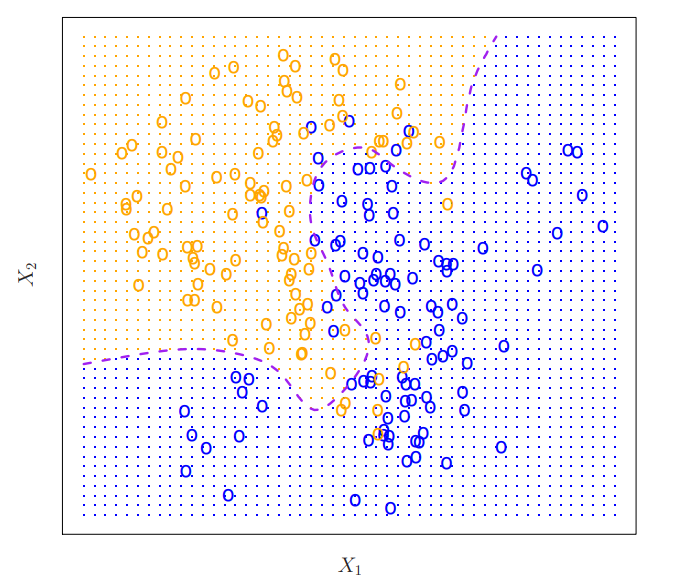
\includegraphics[width=2.83333in,height=\textheight]{images/figura9.png}

}

\caption{FIGURA 9. Un conjunto de datos simulados compuesto por 100
observaciones en cada uno de dos grupos, indicados en azul y en naranja.
La línea discontinua morada representa el límite de decisión de Bayes.}

\end{figure}

\hypertarget{k-nearest-neighbors}{%
\subsubsection{\texorpdfstring{\textbf{K-Nearest
Neighbors}}{K-Nearest Neighbors}}\label{k-nearest-neighbors}}

Los clasificadores de Bayes son buenos para predecir respuestas
cualitativas, pero en realidad no conocemos la distribución condicional
de Y dada X, por lo que no se puede calcular. Como tal, es un estándar
de oro inalcanzable contra el cual comparar otros métodos.

~Uno de estos métodos es el K-vecino más cercano (KNN), que estima la
distribución condicional de Y dada X y clasifica las observaciones dadas
según la clase con la probabilidad estimada más alta. Dado un entero K y
una observación de prueba x0, el clasificador KNN identifica K puntos en
los datos de entrenamiento que están más cerca de x0 y estima la
probabilidad condicional de la clase j como la fracción N0 de puntos con
un valor de respuesta igual A J.

A continuación, estima la probabilidad condicional de la clase j como la
fracción de puntos en N0 cuyos valores de respuesta son iguales a j:

\begin{figure}

{\centering 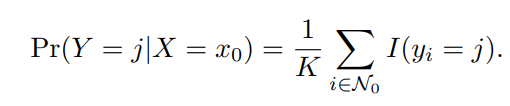
\includegraphics[width=2.55208in,height=\textheight]{images/figura10.png}

}

\end{figure}

El éxito de cualquier método de aprendizaje estadístico depende de
elegir el nivel adecuado de flexibilidad tanto en la regresión como en
la clasificación.

~Esto implica lograr un equilibrio entre el sesgo y la varianza, lo que
puede ser difícil debido a la forma de U del error de prueba.

\hypertarget{capuxedtulo-3-regresiuxf3n-lineal}{%
\subsection{\texorpdfstring{\textbf{Capítulo 3: Regresión
Lineal}}{Capítulo 3: Regresión Lineal}}\label{capuxedtulo-3-regresiuxf3n-lineal}}

La regresión lineal es una herramienta útil para predecir una respuesta
cuantitativa

\hypertarget{regresiuxf3n-lineal-simple}{%
\subsubsection{\texorpdfstring{\textbf{Regresión lineal
simple}}{Regresión lineal simple}}\label{regresiuxf3n-lineal-simple}}

La regresión lineal simple se enfoca para predecir una respuesta
cuantitativa Y en función de una única variable predictora X. Supone que
existe una relación aproximadamente lineal entre X e Y y se puede
escribir esta relación matemáticamente como a continuación:

\begin{itemize}
\tightlist
\item
  \emph{Relación lineal: Y ≈ β0 + β1X}
\end{itemize}

\hypertarget{estimaciuxf3n-de-los-coeficientes}{%
\subsubsection{\texorpdfstring{\textbf{Estimación de los
coeficientes}}{Estimación de los coeficientes}}\label{estimaciuxf3n-de-los-coeficientes}}

En la práctica, β0 y β1 son desconocidos. Así que antes de poder
utilizar Y ≈ β0 + β1X para hacer

predicciones, debemos utilizar datos para estimar los coeficientes. Sea

\emph{(x1, y1), (x2, y2),..., (xn, yn)}

Representan n pares de observaciones, cada uno de los cuales consiste en
una medición de X y una medición de Y.

\begin{itemize}
\tightlist
\item
  Ejemplo: De publicidad, el conjunto de datos consiste en presupuestos
  de publicidad Televisión y ventas de productos para n=200 mercados
  diferentes. El objetivo es obtener los coeficientes de la ecuación
  lineal (3.1) para ajustar bien los datos disponibles. Esto se logra
  encontrando la intersección y la pendiente que el permitan dibujar una
  línea lo más cerca posible de los 200 puntos de datos. Para medir esta
  cercanía se utiliza el criterio de mínimos cuadrados, que se explica
  en este capítulo.
\end{itemize}

\begin{figure}

{\centering 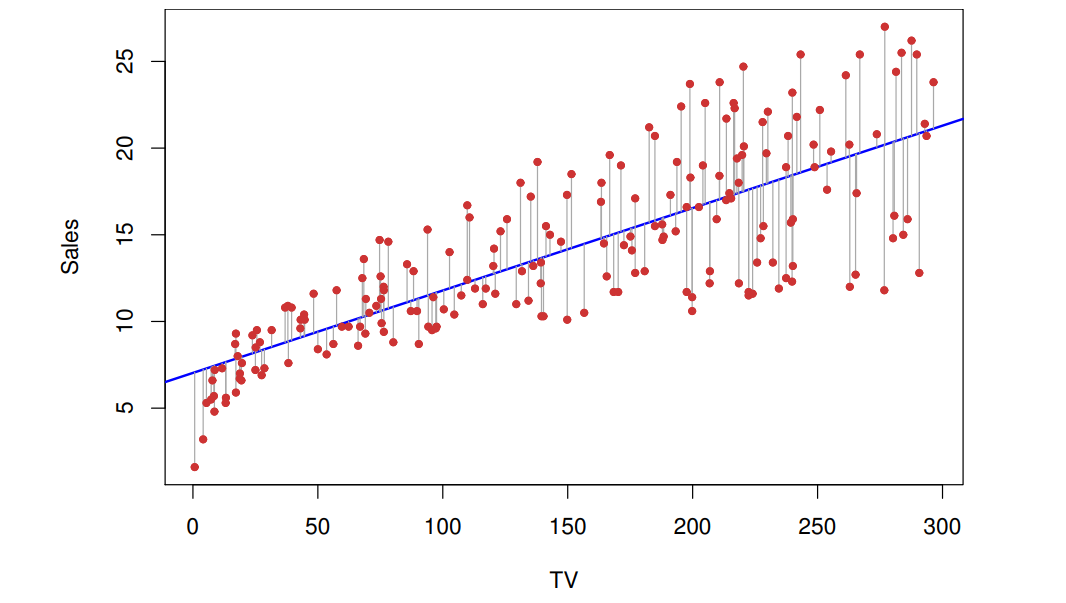
\includegraphics[width=4.125in,height=\textheight]{images/figura11.png}

}

\caption{FIGURA 11. Para los datos de publicidad, se muestra el ajuste
por mínimos cuadrados de la regresión de las ventas en la televisión. El
ajuste se obtiene minimizando la suma de cuadrados residuales.
cuadrados.}

\end{figure}

\hypertarget{evaluaciuxf3n-de-la-precisiuxf3n-de-las-estimaciones-del-coeficiente}{%
\subsubsection{\texorpdfstring{\textbf{Evaluación de la precisión de las
estimaciones del
coeficiente}}{Evaluación de la precisión de las estimaciones del coeficiente}}\label{evaluaciuxf3n-de-la-precisiuxf3n-de-las-estimaciones-del-coeficiente}}

Si f debe aproximarse mediante una función lineal, podemos escribir esta
relación como:

Y = β0 + β1X + ϵ

\begin{itemize}
\item
  β0 es el término de intercepción, es decir, el valor esperado de Y
  cuando X = 0.
\item
  β1 es la pendiente, es decir, el aumento medio de Y asociado a un
  aumento de una unidad en X.
\item
  El término de error es un cajón de sastre para lo que no vemos con
  este método: la verdadera relación probablemente no sea lineal, puede
  haber otras variables que causen variación en Y , y puede haber error
  de medición.
\item
  Normalmente suponemos que el término de error es independiente de X.
\end{itemize}

\begin{figure}

{\centering 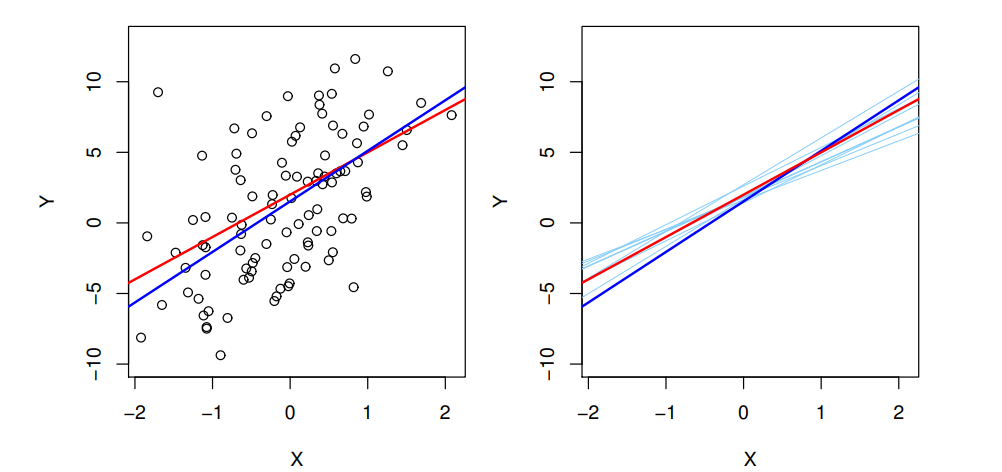
\includegraphics[width=4.11458in,height=\textheight]{images/figura12.png}

}

\caption{Figura 12. Un conjunto de datos simulados. Izquierda: La línea
roja representa la relación verdadera, f(X)=2+3X, que se conoce como
línea de regresión poblacional. La línea azul es la línea de mínimos
cuadrados; es la estimación de mínimos cuadrados para f(X) basada en los
datos observados, mostrados en negro.}

\end{figure}

\hypertarget{evaluaciuxf3n-de-la-precisiuxf3n-del-modelo}{%
\subsubsection{\texorpdfstring{\textbf{Evaluación de la precisión del
modelo}}{Evaluación de la precisión del modelo}}\label{evaluaciuxf3n-de-la-precisiuxf3n-del-modelo}}

Una vez rechazada la hipótesis nula en favor de la hipótesis
alternativa, es natural querer cuantificar en qué medida el modelo se
ajusta a los datos.

La calidad del ajuste de una regresión lineal suele evaluarse mediante
dos magnitudes relacionadas: el error estándar residual (RSE) y el R2.

\hypertarget{error-estuxe1ndar-residual}{%
\subsubsection{\texorpdfstring{\textbf{Error estándar
residual}}{Error estándar residual}}\label{error-estuxe1ndar-residual}}

Hay un término de error ϵ. Debido a la presencia de estos términos de
error, aunque conociéramos la verdadera recta de regresión (es decir,
aunque se conocieran β0 y β1), no podríamos predecir perfectamente Y a
partir de X.

\begin{figure}

{\centering 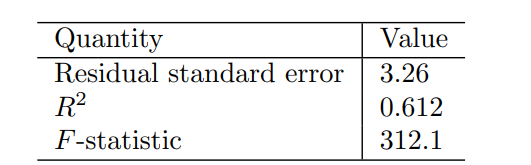
\includegraphics[width=3.01042in,height=\textheight]{images/fig13.png}

}

\end{figure}

El RSE es una estimación de la desviación típica de ϵ. A grandes rasgos,
es la cantidad media en que la respuesta se desviará de la verdadera
línea de regresión.

~\textbf{Se calcula mediante la fórmula:}

\begin{figure}

{\centering 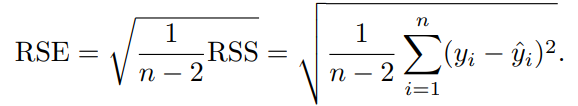
\includegraphics[width=2.77083in,height=\textheight]{images/fig14.png}

}

\end{figure}

\hypertarget{estaduxedstica-r2}{%
\subsubsection{\texorpdfstring{\textbf{Estadística
R2}}{Estadística R2}}\label{estaduxedstica-r2}}

El RSE proporciona una medida absoluta de la falta de ajuste del modelo
a los datos. Pero como se mide en unidades de Y, no siempre está claro
qué es un buen RSE.

El estadístico R2 proporciona una medida alternativa de ajuste. Adopta
la forma de una proporción (la proporción de varianza explicada), por lo
que siempre toma un valor entre 0 y 1, y es independiente de la escala
de Y.

\emph{Para calcular R2, utilizamos la fórmula:}

\begin{figure}

{\centering 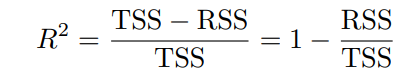
\includegraphics[width=2.15625in,height=\textheight]{images/fig15.png}

}

\end{figure}

El estadístico R2 tiene una ventaja explicativa sobre el error estándar
del residual (SSR) en que, a diferencia del RSE, siempre está entre 0 y
1. Sin embargo, sigue siendo difícil determinar qué es un buen valor
para R2 y generalmente dependerá del uso particular.

Por ejemplo, en algunos problemas de física, se sabe que los datos en
realidad provienen de un modelo lineal con residuos muy pequeños. En
este caso, esperaría que un valor de R2 estuviera muy cerca de 1,
mientras que un valor de R2 mucho más bajo podría indicar un problema
grave en el experimento que generó los datos.

\hypertarget{regresiuxf3n-lineal-muxfaltiple}{%
\subsubsection{\texorpdfstring{\textbf{Regresión lineal
múltiple}}{Regresión lineal múltiple}}\label{regresiuxf3n-lineal-muxfaltiple}}

Con la regresión lineal simple, la respuesta se puede predecir a partir
de una sola variable predictora, pero en la práctica suele haber más de
una.

Se puede realizar una regresión lineal simple para cada predictor para
este propósito, pero no es del todo satisfactoria porque no permite un
predictor y cada ecuación de regresión ignora los otros predictores.

Por el contrario, los modelos de regresión lineal simple se pueden
ampliar para adaptarse a múltiples predictores al proporcionar
coeficientes de pendiente separados para cada predictor en un solo
modelo.

El modelo de regresión lineal adopta la forma:

Y = β0 + β1X1 + β2X2 + -\/-\/- + βpXp + ϵ, (3.19)

Xj representa el j-ésimo predictor y βj cuantifica la asociación entre
esa variable y la respuesta.

Interpretamos βj como el efecto medio efecto

\hypertarget{estimaciuxf3n-de-los-coeficientes-de-regresiuxf3n}{%
\subsubsection{\texorpdfstring{\textbf{Estimación de los coeficientes de
regresión}}{Estimación de los coeficientes de regresión}}\label{estimaciuxf3n-de-los-coeficientes-de-regresiuxf3n}}

Como en el caso de la regresión lineal simple, los coeficientes de
regresión β0, β1,..., βp en (3.19) son desconocidos y deben estimarse.
Dada las estimaciones βˆ0, βˆ1,..., βˆp, podemos hacer predicciones
utilizando la fórmula:

yˆ = βˆ0 + βˆ1x1 + βˆ2x2 + -\/-\/- + βˆpxp

Los parámetros se estiman utilizando el mismo enfoque de mínimos
cuadrados que vimos en el contexto de la regresión lineal simple.
Elegimos β0, β1,..., βp para minimizar la suma de los residuos al
cuadrado:

\begin{figure}

{\centering 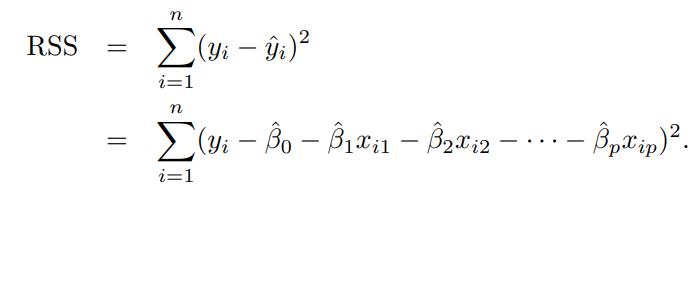
\includegraphics[width=2.42708in,height=\textheight]{images/fig16.png}

}

\end{figure}

Ejemplo de ajuste de mínimos cuadrados a un conjunto de datos con dos
predictores.

\begin{figure}

{\centering 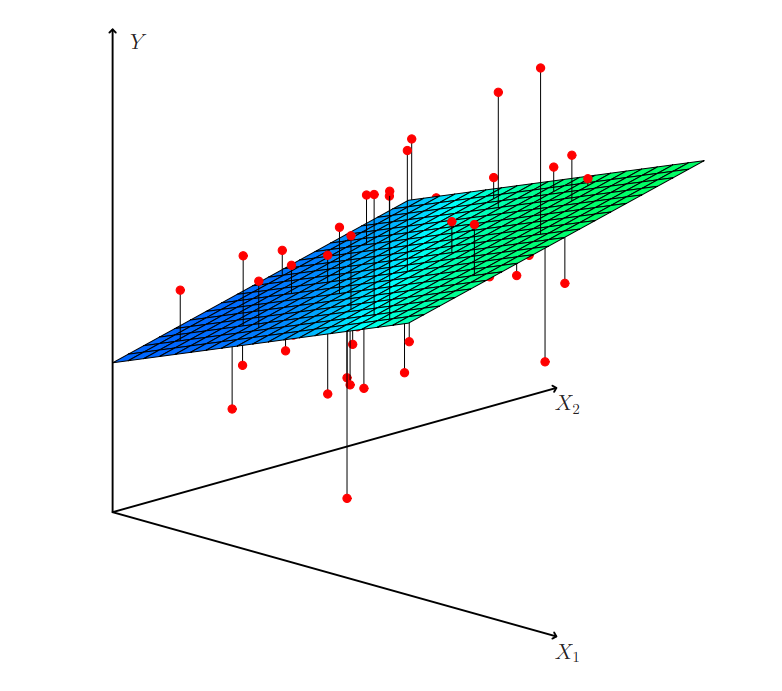
\includegraphics[width=3.35417in,height=\textheight]{images/fig17.png}

}

\caption{Figura 17. En un entorno tridimensional, con dos predictores y
una respuesta, la línea de regresión por mínimos cuadrados se convierte
en un plano.}

\end{figure}

Los coeficientes que minimizan la ecuación son los estimados de los
coeficientes de regresión de mínimos cuadrados múltiples. Estos
estimados tienen formas complicadas que son más fácilmente representadas
mediante álgebra matricial.

\hypertarget{algunas-cuestiones-importantes}{%
\subsubsection{\texorpdfstring{\textbf{Algunas cuestiones
importantes}}{Algunas cuestiones importantes}}\label{algunas-cuestiones-importantes}}

Cuando realizamos una regresión lineal múltiple, normalmente nos
interesa responder a algunas preguntas importantes.

\begin{enumerate}
\def\labelenumi{\arabic{enumi}.}
\item
  ¿Es útil al menos uno de los predictores X1, X2,...,Xp para predecir
  la respuesta?
\item
  ¿Ayudan todos los predictores a explicar Y o sólo es útil un
  subconjunto de los predictores?
\item
  ¿En qué medida se ajusta el modelo a los datos?
\item
  Dado un conjunto de valores predictores, ¿qué valor de respuesta
  deberíamos predecir?
\item
  ¿Cuál es la precisión de nuestra predicción?
\end{enumerate}

\hypertarget{existe-una-relaciuxf3n-entre-la-respuesta-y-los-predictores}{%
\paragraph{\texorpdfstring{\textbf{¿Existe una relación entre la
respuesta y los
predictores?}}{¿Existe una relación entre la respuesta y los predictores?}}\label{existe-una-relaciuxf3n-entre-la-respuesta-y-los-predictores}}

En el marco de la regresión lineal simple, para determinar relación
entre la respuesta y el predictor, basta con comprobar si β1 = 0.

Podemos simplemente comprobar si β1 = 0. En el escenario de regresión
múltiple con p predictores, tenemos que preguntarnos si todos los
coeficientes de regresión son cero, es decir, si β1 = β2 = -\/-\/- = βp
= 0.

Como en la regresión lineal simple, utilizamos una prueba de hipótesis
para responder a esta pregunta. Probamos la hipótesis nula

H0 : β1 = β2 = -\/-\/- = βp = 0

Frente a la alternativa Ha : al menos una βj es distinta de cero.

Esta prueba de hipótesis se realiza calculando el estadístico F, con lo
siguiente:

\begin{figure}

{\centering 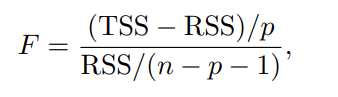
\includegraphics[width=1.71875in,height=\textheight]{images/fig18.png}

}

\end{figure}

\begin{itemize}
\item
  Usar el estadístico F para probar cualquier relación entre el
  predictor y la respuesta es válido cuando p es relativamente pequeño y
  ciertamente pequeño en comparación con n.~Pero a veces tenemos muchas
  variables. Si p\textgreater n, entonces hay más coeficientes βj para
  estimar que observaciones para estimarlos.
\item
  En este caso, ni siquiera podemos ajustar Uno modelo de regresión
  lineal múltiple Usando mínimos cuadrados, por lo que no podemos usar
  el estadístico F ni la mayoría de los otros conceptos que hemos visto
  hasta ahora en este capítulo.
\item
  Sí p es grande, se pueden usar algunos de los métodos discutidos en la
  siguiente sección, como la selección hacia adelante.
\end{itemize}

\hypertarget{variables-importantes}{%
\paragraph{\texorpdfstring{\textbf{Variables
importantes}}{Variables importantes}}\label{variables-importantes}}

El capítulo presenta tres técnicas para la selección de variables en
modelos de regresión múltiple:

\begin{itemize}
\tightlist
\item
  \emph{Selección hacia adelante, selección hacia atrás y selección
  mixta.}
\end{itemize}

En la selección directa, comenzamos con Uno modelo vacío y agregamos un
predictor que minimiza el RSS. A continuación, agregue las variables
predictoras que reducen el RSS al nuevo modelo bivariado. Este proceso
continúa hasta que se cumple la regla de parada.

Con la selección posterior comenzamos con todos los predictores y
eliminamos el predictor con el mayor valor de p, es decir, el predictor
menos estadísticamente significativo. Este proceso continúa hasta que se
cumple la regla de parada.

La selección mixta es una combinación de selección positiva y negativa.
Comenzamos sin predictores en el modelo y agregamos predictores que
brindan el mejor ajuste. Continuamos agregando predictores uno a la vez,
y si en algún momento el valor p de un predictor aumenta más de un
cierto umbral, ese predictor se elimina del modelo. Continuamos haciendo
esto de un lado a otro hasta que todos los predictores en el modelo
tengan valores p suficientemente bajos y todos los predictores fuera del
modelo tengan valores p altos si se agregan al modelo.

\hypertarget{predicciones}{%
\paragraph{\texorpdfstring{\textbf{Predicciones}}{Predicciones}}\label{predicciones}}

Una vez que hemos ajustado el modelo de regresión múltiple. Para
predecir la respuesta Y a partir de un conjunto de valores de los
predictores X1, X2, ...,Xp.

Sin embargo, hay tres tipos de incertidumbre asociada a esta predicción.

Las estimaciones de los coeficientes βˆ0, βˆ1,..., βˆp son estimaciones
de β0, β1,..., βp.

Es decir, el plano de mínimos cuadrados

\emph{Yˆ = βˆ0 + βˆ1X1 + -\/-\/- + βˆpXp}

Es sólo una estimación del verdadero plano de regresión de la población

\emph{f(X) = β0 + β1X1 + -\/-\/- + βpXp.}

La inexactitud de las estimaciones de los coeficientes está relacionada
con el error reducible.

Podemos calcular un intervalo de confianza para determinar lo cerca que
estará \emph{Yˆ de f(X).}

En la práctica, asumir que un modelo lineal de f(X) eso casi siempre una
aproximación de la realidad introduce una fuente adicional de error
potencialmente reducible llamada sesgo del modelo. Usando el modelo
lineal, estimamos la mejor aproximación lineal de la superficie real.
Pero aquí ignoramos esta diferencia y actuamos como si el modelo lineal
fuera correcto.

\hypertarget{predictores-cualitativos}{%
\subsubsection{\texorpdfstring{\textbf{Predictores
cualitativos}}{Predictores cualitativos}}\label{predictores-cualitativos}}

Los predictores cualitativos se representan como variables ficticias en
la tabla de datos. Describe cómo usar estas variables ficticias para
modelar las relaciones entre los predictores cualitativos y las
respuestas. Además, existen consideraciones especiales para el ajuste de
modelos con predictores cuantitativos y cualitativos, incluida la
interpretación de coeficientes.

\hypertarget{predictores-con-suxf3lo-dos-niveles}{%
\paragraph{\texorpdfstring{\textbf{Predictores con sólo dos
niveles}}{Predictores con sólo dos niveles}}\label{predictores-con-suxf3lo-dos-niveles}}

Si deseamos investigar las diferencias en el saldo de la tarjeta de
crédito entre aquellos que poseen una casa y aquellos que no, podemos
incorporar un predictor cualitativo o factor en nuestro modelo de
regresión.

Si el factor solo tiene dos niveles o valores posibles, entonces es muy
simple incorporarlo en el modelo. Simplemente creamos una variable
indicadora o variable dummy que toma dos posibles valores numéricos.

Por ejemplo, en base a la variable own, podemos crear una nueva variable
que tome la siguiente forma:

\begin{figure}

{\centering 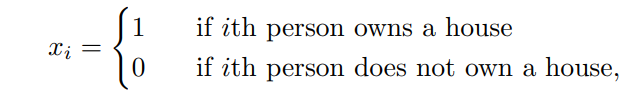
\includegraphics[width=3.46875in,height=\textheight]{images/f19.png}

}

\end{figure}

Utilizar esta variable como predictor en la ecuación de regresión. El
resultado en el modelo:

\begin{figure}

{\centering 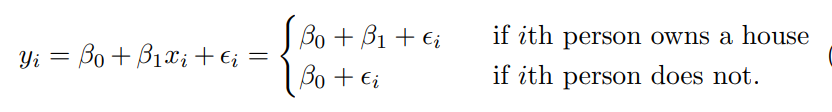
\includegraphics[width=3.67708in,height=0.48958in]{images/f20.png}

}

\end{figure}

La figura 21 muestra el conjunto de datos de crédito contiene
información sobre el saldo, la edad

tarjetas, educación, ingresos, límite y calificación de una serie de
clientes potenciales

\begin{figure}

{\centering 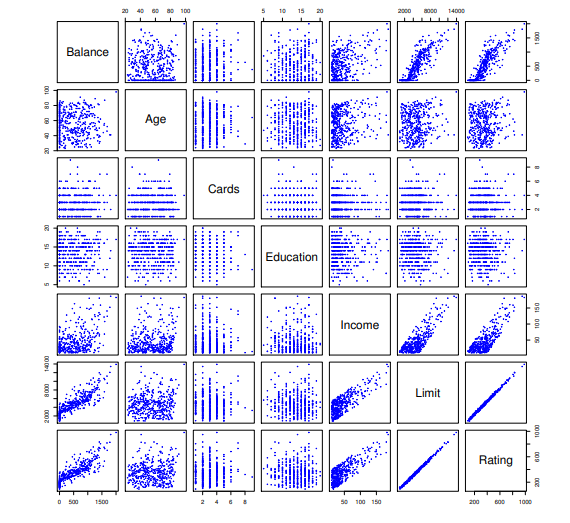
\includegraphics[width=3.20833in,height=\textheight]{images/f21.png}

}

\caption{Figura 21. Datos credito}

\end{figure}

\hypertarget{predictores-cualitativos-con-muxe1s-de-dos-niveles}{%
\paragraph{\texorpdfstring{\textbf{Predictores cualitativos con más de
dos
niveles}}{Predictores cualitativos con más de dos niveles}}\label{predictores-cualitativos-con-muxe1s-de-dos-niveles}}

Cuando un predictor cualitativo tiene más de dos niveles, una única
variable ficticia no puede representar todos los valores posibles.

No puede representar todos los valores posibles. En esta situación, se
debe crear variables ficticias adicionales.



\end{document}
